\subsection{How to represent weights?}
When it comes to the object-oriented implementation of neural networks, this is probably the most important question that has to be answered. Should weights belong to the neuron? If yes, should it be the sending or the receiving neuron? Or maybe they should belong to a layer? Or maybe to the whole network? Maybe we should even implement them as separate objects?

Being a feedforward network with only one layer, and therefore having no weights that connect two neurons, single-layer perceptron simplifies this problem. Basically, we have three options:
\begin{enumerate}
  \item Input weights of each neuron are stored as a vector inside that neuron.
  \item The matrix of all input weights is stored in the network.
  \item The weights are implemented as objects and connected to neurons.
\end{enumerate}

Second option is the most efficient (vector-matrix multiplication), but not very object-oriented. What is neuron in this implementation? Clearly, the network is just a matrix of weights + some learning rules. Should the neuron be an activation function with a learning rate? But then again, storing them in the network would be even more efficient. So basically, we don’t need a Neuron class. All we need is a matrix and several functions for manipulating it. That doesn’t sound object-oriented to me.

Third option in this case would be an over-engineering. It would just make the whole thing way more complicated. Implementing weights as objects would probably make some sense in a multi-layer neural network, where each weight is a connection between two neurons (we can think of inputs as of fake neurons). It connects two neurons, sends a signal between them and has a “strength” which can be updated. As a result, neurons would not know about other neurons. They would just receive, process, and emit the signals. I assume that such implementation would not be very fast, but it could be used for modeling purposes. I will write more about this idea in a post dedicated to multi-layer networks.

First option looks like most appropriate for single-layer perceptrons. And it’s very easy to implement, so I’ll stick to it.

\subsection{Activation functions}
There are two ways of representing activation functions in this project:

\begin{enumerate}
  \item Implement them as methods
  \item Implement them as classes
\end{enumerate}

The first approach will be faster and consume less memory. We create a base class Neuron with abstract methods activation and activationDerivative. Each subclass will be a special type of neuron, such as BinaryThresholdNeuron, SigmoidNeuron, that implements a corresponding activation function.

\begin{figure}[H]
  \centering
  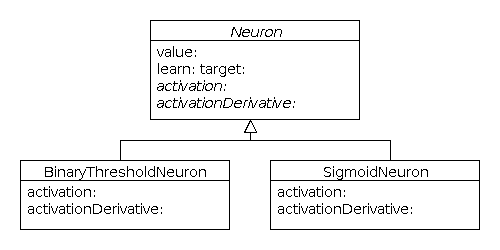
\includegraphics[width=0.8\linewidth]{activation1}
  \caption{Implementing activation functions as methods of specific subclasses on Neuron}
  \label{fig:activation1}
\end{figure}

Another way of implementing activations is to create a base class ActivationFunction with two abstract methods, value: and derivative:. This approach is more flexible, because if someone wants to use a new activation function, he will be able to implement it as a subclass, only defining what it is and what is its derivative. Then he will be able to pass an object of this class to an existing neuron. It doesn’t seem logical to reimplement the whole neuron every time we need to create a function.

\begin{figure}[H]
  \centering
  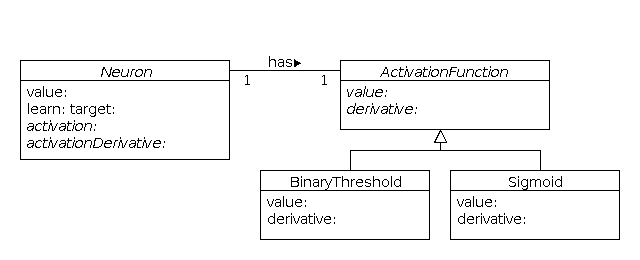
\includegraphics[width=0.9\linewidth]{activation2}
  \caption{Implementing activation functions as separate classes}
  \label{fig:activation2}
\end{figure}

So the real question can sound like this:
\textit{Are neurons defined by their activations? Does having a different activation means being a completely different type of neuron?}

\subsection{Shared or separate activation and learning rate?}
Both activation and learning rate can be either shared by all neurons of a perceptron or be stored separately in each neuron.The question is: do we need to have neurons with different activations and different learning rates?

Let’s assume that we don’t. Indeed, in most cases all neurons of a network (or a layer) share the same learning rate and have the same activation. If the network has many neurons (and most networks do), then we will be storing the same number just as many times. And if the activation function is implemented as a class, then we will be creating a separate instance of that class for each neuron.

However, if we wanted to parallelize the computations done by neurons, it would be better to have a separate learning rate and separate activation for each neuron (or each block of neurons). Otherwise they will just block each other trying to access the shared memory on every single step. And besides, the total memory occupied by this “heavy” neuron would still be rather small. I think, such neuron (or a group of them) would easily fit in the local memory of a single core of GPU.

But single-layer perceptrons do not usually perform heavy computations. They are more useful for the modeling purposes. That’s why we should probably take the “separate” approach and allow the user to build a network out of completely different neurons (like building blocks).

By the way, for multi-layer network the nice idea would be to share the same activation and learning rate inside one layer, but allow user to have completely different layers. In the end, he should be able to build some complicated network like the convolutional network on the picture. But that’s not the topic of this post.

\begin{figure}[H]
  \centering
  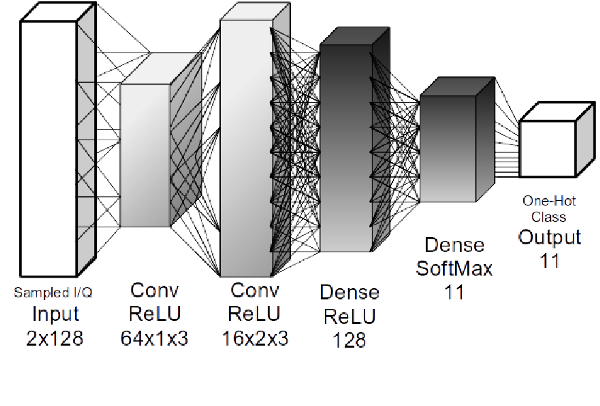
\includegraphics[width=0.8\linewidth]{conv}
  \caption{A convolutional neural network with four hidden layers}
  \label{fig:conv}
\end{figure}

\subsection{Data shuffling}
Online perceptrons are sensitive to the order in which training examples are received. Weight updates are made after each training example, that’s why the training vectors \#(\#(0 1) \#(1 1)) and \#(\#(1 1) \#(0 1)) will result in different weight vectors. Depending on the order of examples, the perceptron may need a different number of iterations to converge.

That’s why, to test the complexity of such learning, the perceptron has to be trained by examples randomly selected from a training set.
